\subsection{XmlBuffer}
XmlBuffer har til ansvar at tage imod en strøm af data fra en socketforbindelse og opdele XML-dokumenter. Den fungerer ved, at når en klient har modtaget data fra en socket tilføjes dette data til bufferen via AddData(). Herefter kaldes GetDocuments(), som returnerer en liste over de komplette XML-dokumenter, bufferen indeholder. De returnerede dokumenter fjernes derefter fra bufferen.\\

Der blev derudover oprettet et interface, IProtocolBuffer, dette var i tilfælde af at systemet senere skulle udvides med flere buffere, så systemet ville kunne kommunikere med flere/andre dataformater.

\begin{figure}[H]
	\centering
	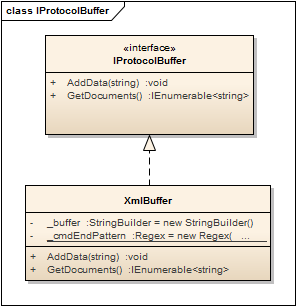
\includegraphics[width=0.4\textwidth]{Systemdesign/SharedLib/Images/Klasser/IProtocolBuffer.png}
	\caption{XmlBuffer der implementerer IProtocolBuffer}
	\label{fig:klasseXmlBuf}
\end{figure}
